%To compile as handout, use
%pdflatex "\def\ishandout{1} \input{filename.tex}"
%Defaults to non-handout mode (with slide reveals)
\ifdefined\ishandout
  \documentclass[handout]{beamer}
\else
  \documentclass{beamer}
\fi
 
\usepackage{econ103slides} 

\date{Lecture \# 6}
\begin{document} 




%%%%%%%%%%%%%%%%%%%%%%%%%%%%%%%%%%%%%%%%

\begin{frame}[plain]
	\titlepage 
	

\end{frame} 

%%%%%%%%%%%%%%%%%%%%%%%%%%%%%%%%%%%%%%%%

\begin{frame}

\begin{center}
 \Huge Basic Probability -- Part II
\end{center}

\end{frame}
%%%%%%%%%%%%%%%%%%%%%%%%%%%%%%%%%%%%%%%%%
%
%\begin{frame}
%
%\centering \Huge Classical Probability Examples Where Order Doesn't Matter
%
%\end{frame}
%%%%%%%%%%%%%%%%%%%%%%%%%%%%%%%%%%%%%%%%%
%
%\begin{frame}
%
%\frametitle{Poker -- Deal 5 Cards, Order Doesn't Matter}
%
%\begin{block}{Basic Outcomes}
%\vspace{0.3em} \pause
%$\displaystyle{52 \choose 5}$ possible hands
%\end{block}\pause
%\begin{block}{How Many Hands have Four Aces? \hfill 
\includegraphics[scale = 0.05]{./images/clicker} } \pause
%\alert{48 (\# of ways to choose the single card that is not an ace)}
%\end{block}\pause
%
%\begin{block}{What is the Probability of Getting Four Aces?}
%\vspace{0.3em} \pause
%$48/\displaystyle{52 \choose 5}$
%\end{block}
%
%
%\end{frame}
%%%%%%%%%%%%%%%%%%%%%%%%%%%%%%%%%%%%%%%%%
%\begin{frame}
%\frametitle{Poker -- Deal 5 Cards, Order Doesn't Matter}
%\begin{block}{How Many Hands have Four of a Kind?\hfill 
\includegraphics[scale = 0.05]{./images/clicker} }\pause
%	\begin{itemize}
%		\item 13 ways to choose \emph{which} card we have four of \pause
%		\item 48 ways to choose the last card in the hand \pause
%		\item $13 \times 48 = \alert{624}$ \pause
%	\end{itemize}
%\end{block}
%\begin{block}{What is the Probability of Being Dealt 4 of a Kind?}
%\vspace{0.3em} \pause
%$624/\displaystyle{52 \choose 5}$
%\end{block}
%\vspace{8em}
%
%\end{frame}
%%%%%%%%%%%%%%%%%%%%%%%%%%%%%%%%%%%%%%%%%
%\begin{frame}
%
%\centering \Huge Even if the basic outcomes are equally likely, the events of interest may not be...
%
%
%\end{frame}
%%%%%%%%%%%%%%%%%%%%%%%%%%%%%%%%%%%%%%%%%
%\begin{frame}
%\frametitle{``Odd Question'' \# 4}
%To throw a total of 7 with a pair of dice, you have to get a 1 and a 6, or a 2 and a 5, or a 3 and a 4.
%To throw a total of 6 with a pair of dice, you have to get a 1 and a 5, or a 2 and a 4, or a 3 and another 3.
%	\vspace{1em}
%	With two fair dice, you would expect:
%		\begin{enumerate}[(a)]
%			\item To throw 7 more frequently than 6.
%			\item To throw six more frequently than 7.
%			\item To throw 6 and 7 equally often.
%		\end{enumerate}
%\end{frame}
%%%%%%%%%%%%%%%%%%%%%%%%%%%%%%%%%%%%%%%%%
%\begin{frame}
%\frametitle{Basic Outcomes Equally Likely, Events of Interest Aren't}
%
%\begin{table}
%	\begin{tabular}{|lr|cccccc|}
%	\hline
%	&&\multicolumn{6}{|c|}{Second Die}\\
%	&&1&2&3&4&5&6\\
%	\hline
%	&1&2&3&4&5&\alert{6}&\textcolor{blue}{7}\\
%	&2&3&4&5&\alert{6}&\textcolor{blue}{7}&8\\
%	First&3&4&5&\alert{6}&\textcolor{blue}{7}&8&9\\
%	Die&4&5&\alert{6}&\textcolor{blue}{7}&8&9&10\\
%	&5&\alert{6}&\textcolor{blue}{7}&8&9&10&11\\
%	&6&\textcolor{blue}{7}&8&9&10&11&12\\
%	\hline
%	\end{tabular}
%	\caption{There are 36 equally likely basic outcomes, of which 5 correspond to a sum of six and 6 correspond to a sum of  seven.}
%\end{table}
%	\alert{$P(7) = 6/36 = 1/6$}\\
%	\alert{$P(6) = 5/36$}
%\end{frame}
%%%%%%%%%%%%%%%%%%%%%%%%%%%%%%%%%%%%%%%%%
\begin{frame}

\begin{center}\Huge Derive Rules for Computing Probabilities from Axioms\end{center}
\end{frame}
%%%%%%%%%%%%%%%%%%%%%%%%%%%%%%%%%%%%%%%%
\begin{frame}
\frametitle{Recall: Axioms of Probability}

Let $S$ be the sample space. With each event $A \subseteq S$ we associate a real number $P(A)$ called the \alert{probability of $A$}, satisfying the following conditions:
\vspace{1em}
\begin{description}
	\item[Axiom 1] $0 \leq P(A) \leq 1$ 
	\item[Axiom 2] $P(S)=1$
	\item[Axiom 3] If $A_1, A_2, A_3, \hdots$ are mutually exclusive events, then $P(A_1\cup A_2 \cup A_3 \cup \cdots) = P(A_1) + P(A_2) + P(A_3) + \hdots$
\end{description}

\end{frame}
%%%%%%%%%%%%%%%%%%%%%%%%%%%%%%%%%%%%%%%%
\begin{frame}
\frametitle{Key Point}
The axoims of probability are out \emph{\alert{starting assumptions}} -- they are a complete description what we \emph{\alert{mean}} when we say ``probability.'' We use the axioms to derive various results for \emph{\alert{computing}} probabilities.
\end{frame}

%%%%%%%%%%%%%%%%%%%%%%%%%%%%%%%%%%%%%%%%
%Some macros for the Venn Diagrams
\def\EventA{(-0.35,0) circle (1.2)}
\def\EventB{(1.35,0) circle (1.2)}
\def\EventC{(-0.35,0) circle (0.6)}
\def\EventD{(0,0) circle (1.6)}
\def\SampleSpace{(-2,-2) rectangle (3,2)}
%%%%%%%%%%%%%%%%%%%%%%%%%%%%%%%%%%%%%%%%
\begin{frame}
	\frametitle{The Complement Rule: $P(A^c) = 1- P(A)$}
	\begin{columns}
	
\column{0.7\textwidth}
\uncover<2->{Since $A, A^c$ are mutually exclusive and collectively exhaustive:}
$$\uncover<3->{P(A \cup A^c) =} \uncover<4->{P(A) + P(A^c) =} \uncover<5->{P(S) =} \uncover<6->{1}$$
\uncover<7->{Rearranging:}
	\uncover<8->{$$P(A^c) = 1 - P(A)$$}
\column{0.3\textwidth}
\uncover<1->{
\begin{figure}
\centering
\begin{tikzpicture}[scale = 0.6]
	\draw (1.8,0.8) node [above]{$A^c$};
	\draw \EventA node [above] {$A$};
      \draw \SampleSpace node [text=black,above] {$S$};
\end{tikzpicture}
\caption{$A\cap A^c = \emptyset$, $A \cup A^c = S$}
\end{figure}}

\end{columns}
\end{frame}
%%%%%%%%%%%%%%%%%%%%%%%%%%%%%%%%%%%%%%%%
\begin{frame}
\frametitle{Another Important Rule -- Equivalent Events}

\begin{block}{If A and B are Logically Equivalent, then $P(A) = P(B)$.}\end{block}

\begin{alertblock}{In other words, if A and B contain exactly the same basic outcomes, then $P(A) = P(B)$.}\end{alertblock}

Although this seems obvious it's important to keep in mind, especially later in the course...
\end{frame}
%%%%%%%%%%%%%%%%%%%%%%%%%%%%%%%%%%%%%%%%
\begin{frame}
\frametitle{The Logical Consequence Rule}

\begin{block}{If B Logically Entails A, then $P(B)\leq P(A)$}\end{block}

\begin{alertblock}{In other words, $B\subseteq A \Rightarrow P(B)\leq P(A)$}\end{alertblock}


\begin{block}{Why is this so?}
If $B \subseteq A$, then all the basic outcomes in $B$ are also in $A$.
\end{block}

\end{frame}
%%%%%%%%%%%%%%%%%%%%%%%%%%%%%%%%%%%%%%%%

\begin{frame}
\frametitle{Deriving The Logical Consequence Rule}
	\begin{columns}
	
\column{0.75\textwidth}
\uncover<2->{Since $B \subseteq A$, we have $B = A\cap B$ and $A = B \cup (A \cap B^c)$.}\uncover<3->{ Combining these,
	$$A = (A \cap B) \cup (A \cap B^c)$$}
\uncover<4->{Now since $(A \cap B) \cap (A \cap B^c) = \emptyset$,}
\begin{eqnarray*}
	\uncover<5->{P(A) &=& P(A \cap B)  + P(A \cap B^c)\\}
	\uncover<6->{&=&  P(B) + P(A \cap B^c)\\}
	\uncover<7->{&\geq& P(B)}
\end{eqnarray*}
\uncover<8->{because $0 \leq P(A \cap B^c) \leq 1$.}
\column{0.25\textwidth}
\uncover<1->{\begin{figure}
\centering
\begin{tikzpicture}[scale = 0.55]
	\draw \EventC;
	\draw \EventD;
	\draw (0, 0.5) node [above] {$A$};
	\draw (-0.3, -0.5) node [above] {$B$};
      \draw \SampleSpace node [text=black,above] {$S$};
\end{tikzpicture}
\caption{$B = A\cap B$, and $A = B \cup (A \cap B^c)$}
\end{figure}}

\end{columns}


\end{frame}
%%%%%%%%%%%%%%%%%%%%%%%%%%%%%%%%%%%%%%%%
\begin{frame}
\frametitle{``Odd Question'' \# 2}
\footnotesize
Pia is thirty-one years old, single, outspoken, and smart. She was a philosophy major. When a student, she was an ardent supporter of Native American rights, and she picketed a department store that had no facilities for nursing mothers. Rank the following statements in order from most probable to least probable.

	\vspace{1em}

		\begin{enumerate}[(a)]
			\item Pia is an active feminist.
			\item Pia is a bank teller.
			\item Pia works in a small bookstore.
			\item Pia is a bank teller and an active feminist.
			\item Pia is a bank teller and an active feminist who takes yoga classes.
			\item Pia works in a small bookstore and is an active feminist who takes yoga classes.
		\end{enumerate}
\end{frame}
%%%%%%%%%%%%%%%%%%%%%%%%%%%%%%%%%%%%%%%%
\begin{frame}
\frametitle{``Odd Question'' \# 2 -- Seven \emph{Events}}
Write events D, E, and F in terms of A, B, C, and Y.
		\begin{enumerate}[A]
			\item = Pia is an active feminist.
			\item = Pia is a bank teller.
			\item = Pia works in a small bookstore.
			\item[Y] = Pia takes yoga classes.\vspace{2em}
			\item = Pia is a bank teller and an active feminist \pause \alert{$= A\cap B$}\pause
			\item = Pia is a bank teller and an active feminist who takes yoga classes \pause \alert{$= A \cap B \cap Y$} \pause
			\item = Pia works in a small bookstore and is an active feminist who takes yoga classes \pause \alert{$= A \cap C \cap Y$}
		\end{enumerate}
\end{frame}
%%%%%%%%%%%%%%%%%%%%%%%%%%%%%%%%%%%%%%%%
\begin{frame}
\frametitle{``Odd Question'' \# 2 -- Which Events are Subsets?}
		\begin{enumerate}[A]
			\item = Pia is an active feminist.
			\item = Pia is a bank teller.
			\item = Pia works in a small bookstore.
			\item[Y] = Pia takes yoga classes.\vspace{2em}
			\item $=A\cap B \pause \Rightarrow \alert{D\subseteq A,} \pause \alert{D\subseteq B}$\pause
			\item $=A\cap B \cap Y\pause\Rightarrow \alert{E\subseteq D}$\pause
			\item $=A\cap C \cap Y \pause \Rightarrow \alert{F \subseteq A,} \pause\alert{F \subseteq C}$
		\end{enumerate}
\end{frame}
%%%%%%%%%%%%%%%%%%%%%%%%%%%%%%%%%%%%%%%%
\begin{frame}
\frametitle{``Odd Question'' \# 2 -- Apply Logical Consequence Rule}
		\begin{enumerate}[A]
			\item = Pia is an active feminist.
			\item = Pia is a bank teller.
			\item = Pia works in a small bookstore.
			\item[Y] = Pia takes yoga classes.\vspace{2em}
			\item $=A\cap B  \Rightarrow D\subseteq A, D\subseteq B \pause \Rightarrow \alert{P(D) \leq P(A), \pause P(D) \leq P(B)}$\pause
			\item $=A\cap B \cap Y\Rightarrow E\subseteq D \pause \Rightarrow \alert{P(E) \leq P(D)}$\pause
			\item $=A\cap C \cap Y \Rightarrow F \subseteq A, F \subseteq C \pause \Rightarrow \alert{P(F) \leq P(A), \pause P(F) \leq P(C)}$
		\end{enumerate}
\end{frame}
%%%%%%%%%%%%%%%%%%%%%%%%%%%%%%%%%%%%%%%%
\begin{frame}
\frametitle{``Odd Question'' \# 2 -- Putting These Together...}
 \footnotesize
		\begin{enumerate}[(a)]
			\item Pia is an active feminist.
			\item Pia is a bank teller.
			\item Pia works in a small bookstore.
			\item Pia is a bank teller and an active feminist.
			\item Pia is a bank teller and an active feminist who takes yoga classes.
			\item Pia works in a small bookstore and is an active feminist who takes yoga classes.
		\end{enumerate}
\begin{alertblock}{Any Correct Ranking Must Satisfy:}\end{alertblock}
\begin{eqnarray*}
\mbox{(a)}\geq \mbox{(d)}\geq \mbox{(e)}\\
\mbox{(b)}\geq \mbox{(d)}\geq \mbox{(e)}\\
\mbox{(a)}\geq \mbox{(f)}\\
\mbox{(c)}\geq \mbox{(f)}
\end{eqnarray*}
\end{frame}
%%%%%%%%%%%%%%%%%%%%%%%%%%%%%%%%%%%%%%%%
\begin{frame}
\frametitle{Throw a Fair Die Once}
\begin{block}{$E = $ roll an even number}
\end{block}
\begin{block}{What are the basic outcomes?}\pause
$\{1,2,3,4,5,6\}$
\end{block}\pause
\begin{block}{What is $P(E)$?\hfill 
\includegraphics[scale = 0.05]{./images/clicker} }\pause
$E = \{2,4,6\}$ and the basic outcomes are equally likely (and mutually exclusive), so 
	$$P(E) = 1/6 + 1/6 + 1/6 = 3/6 = \alert{1/2}$$
\end{block}

\end{frame}
%%%%%%%%%%%%%%%%%%%%%%%%%%%%%%%%%%%%%%%%
\begin{frame}
\frametitle{Throw a Fair Die Once}
\begin{block}{$E = $ roll an even number \hfill $M = $ roll a 1 or a prime number}
\end{block}\pause
\begin{alertblock}{What is $P(E\cup M)$?\hfill 
\includegraphics[scale = 0.05]{./images/clicker} }\end{alertblock}
\pause
Key point: $E$ and $M$ are not mutually exclusive! \pause
	\begin{eqnarray*}
		P(E\cup M) &=& P(\{1,2,3,4,5,6\})= 1\\ \pause
		P(E) &=& P(\{2,4,6\}) = 1/2\\ \pause
		P(M) &=& P(\{1,2,3,5\}) = 4/6 = 2/3\\ \\ \pause
		P(E) + P(M) &=& 1/2 + 2/3 = 7/6 \pause \neq P(E\cup M) = 1
	\end{eqnarray*}

\end{frame}
%%%%%%%%%%%%%%%%%%%%%%%%%%%%%%%%%%%%%%%%


\begin{frame}
\frametitle{The Addition Rule -- Don't Double-Count!}
$$P(A\cup B) = P(A) + P(B) - P(A\cap B)$$
\begin{figure}
\centering
\begin{tikzpicture}[scale = 1.2]

	\begin{scope}[fill opacity = 0.5]
		\fill[blue] \EventA;
		\fill[red] \EventB;
	\end{scope}
	
	\draw \EventA node [above] {$A$};
	\draw \EventB node [above] {$B$};
      \draw \SampleSpace node [text=black,right] {$S$};
\end{tikzpicture}
\end{figure}
\alert{Construct a formal proof as an optional homework problem.}
\end{frame}
%%%%%%%%%%%%%%%%%%%%%%%%%%%%%%%%%%%%%%%%
\begin{frame}
\begin{center}\Huge Who's on the other side?\end{center}
\end{frame}
%%%%%%%%%%%%%%%%%%%%%%%%%%%%%%%%%%%%%%%%
\begin{frame}
\frametitle{Three Cards, Each with a Face on the Front and Back}
\begin{figure}
\fbox{
\includegraphics[scale = 0.75]{./images/gaga}}
\hspace{1em}
\fbox{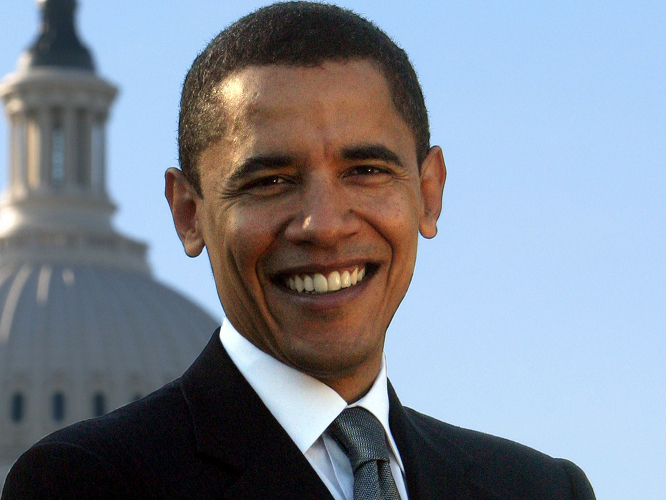
\includegraphics[scale = 0.75]{./images/obama}}
\end{figure}
\begin{enumerate}
	\item Gaga/Gaga
	\item Obama/Gaga
	\item Obama/Obama
\end{enumerate} \pause
\begin{alertblock}{I draw a card at random and look at one side: it's Obama. What is the probability that the other side is also Obama?\\\hfill
\includegraphics[scale = 0.05]{./images/clicker} }\end{alertblock}
\end{frame}
%%%%%%%%%%%%%%%%%%%%%%%%%%%%%%%%%%%%%%%%
\begin{frame}
\frametitle{Let's Try The Method of Monte Carlo...}
\framesubtitle{When you don't know how to calculate, simulate.}
Procedure
\begin{enumerate}
\item Close your eyes and thoroughly shuffle your cards.
\item Keeping eyes closed, draw a card and place it on your desk.
\item Stand if Obama is face-up on your chosen card. 
\item We'll count those standing and call the total $N$
\item Of those standing, sit down if Obama is \emph{not} on the back of your chosen card.
\item We'll count those \emph{still} standing and call the total $m$.
\end{enumerate}

\begin{alertblock}{Monte Carlo Approximation of Desired Probability $\displaystyle= \frac{m}{N}$}\end{alertblock}
\end{frame}
%%%%%%%%%%%%%%%%%%%%%%%%%%%%%%%%%%%%%%%%
\begin{frame}

% Set the overall layout of the tree
\tikzstyle{level 1}=[level distance=3.5cm, sibling distance=3.5cm]
\tikzstyle{level 2}=[level distance=3.5cm, sibling distance=2cm]

% Define styles for bags and leafs
\tikzstyle{bag} = [text width=4em, text centered]
\tikzstyle{end} = [circle, minimum width=3pt,fill, inner sep=0pt]


\begin{tikzpicture}[thick,scale=0.94, every node/.style={transform shape},grow=right]
\node[bag]{Choose Card}
    child {
        node[bag] {Obama Obama}        
        child {
                node[end, label=right:
                    {Obama}] {}
                edge from parent
                node[below]  {$\frac{1}{2}$}
            }
            child {
                node[end, label=right:
                    {Obama}] {}
                edge from parent
                node[above] {$\frac{1}{2}$}
            }
            edge from parent 
            node[below]  {$\frac{1}{3}$}
    }
        child {
        node[bag] {Obama Gaga}        
        child {
                node[end, label=right:
                    {Gaga}] {}
                edge from parent
                node[below]  {$\frac{1}{2}$}
            }
            child {
                node[end, label=right:
                    {Obama}] {}
                edge from parent
                node[above] {$\frac{1}{2}$}
            }
            edge from parent 
            node[above]{$\frac{1}{3}$}
    }
    child {
        node[bag] {Gaga Gaga}        
        child {
                node[end, label=right:
                    {Gaga}] {}
                edge from parent
                node[below]  {$\frac{1}{2}$}
            }
            child {
                node[end, label=right:
                    {Gaga}] {}
                edge from parent
                node[above] {$\frac{1}{2}$}
            }
        edge from parent         
            node[above] {$\frac{1}{3}$}
    };
\end{tikzpicture}

\end{frame}
%%%%%%%%%%%%%%%%%%%%%%%%%%%%%%%%%%%%%%%%
\begin{frame}
\frametitle{Conditional Probability -- Reduced Sample Space}
\framesubtitle{Set of relevant outcomes restricted by condition}
$$P(A|B) = \frac{P(A\cap B)}{P(B)},\;\; \mbox{provided } P(B)>0$$
\begin{figure}
\centering
\begin{tikzpicture}[scale = 1]

	\begin{scope}[fill opacity = 0.5]
		\fill[red] \EventB;
      	\clip \EventA;
      	\fill[blue] \EventB;
    \end{scope}
	\draw \EventA node [above] {$A$};
	\draw \EventB node [above] {$B$};
      \draw \SampleSpace node [right] {$S$};
\end{tikzpicture}
\caption{$B$ becomes the ``new sample space'' so we need to re-scale by $P(B)$ to keep probabilities between zero and one.}
\end{figure}
\end{frame}
%%%%%%%%%%%%%%%%%%%%%%%%%%%%%%%%%%%%%%%%
\begin{frame}
\frametitle{Who's on the other side?}
Let $O_F$ be the event that Obama is on the front of the card of the card we draw and $O_B$ be the event that he is on the back.\pause
$$P(O_B|O_F) = \pause \frac{P(O_B\cap O_F)}{P(O_F)} = \pause \alert{\frac{1/3}{1/2}= \pause 2/3}$$

\end{frame}
%%%%%%%%%%%%%%%%%%%%%%%%%%%%%%%%%%%%%%%%
% \begin{frame}
% \frametitle{Independence and The Multiplication Rule}
% \begin{block}{The Multiplication Rule}
% Just rearrange the definition of conditional probability:
% $P(A\cap B) = P(A|B)P(B)$
% \end{block}\pause
% \begin{block}{Statistical Independence}
% $P(A\cap B) = P(A)P(B)$
% \end{block}\pause
% \begin{alertblock}{By the Multiplication Rule}
% $\mbox{Independence } \iff P(A|B) = P(A)$\\
% \end{alertblock}\pause
% \begin{block}{Interpreting Independence}
% Knowing that $B$ has occurred doesn't give us any additional information about whether $A$ will.
% \end{block}
% \end{frame}
% %%%%%%%%%%%%%%%%%%%%%%%%%%%%%%%%%%%%%%%%

% \begin{frame}
% \frametitle{Will Having 5 Children Guarantee a Boy?}
% A couple plans to have five children. Assuming that each birth is independent and male and female children are equally likely, what is the probability that they have at least one boy?
% \vspace{1em}

% \pause
% \alert{By Independence and the Complement Rule,}
% 	\begin{eqnarray*}
% 		P(\mbox{no boys})&=&\pause P(\mbox{5 girls})\\
% 							&=&\pause 1/2 \times 1/2 \times 1/2 \times 1/2 \times 1/2\\
% 							&=&\pause 1/32\\ \\ \pause
% 		P(\mbox{at least 1 boy})&=&\pause1 - P(\mbox{no boys})\\
% 		&=&\pause1 - 1/32 =\pause 31/32 = 0.97
% 	\end{eqnarray*}

% \end{frame}
% %%%%%%%%%%%%%%%%%%%%%%%%%%%%%%%%%%%%%%%%
%
%\begin{frame}
%\frametitle{An Example -- Do you agree with this calculation?\hfill
\includegraphics[scale = 0.05]{./images/clicker} }
%\begin{quote}
%	On September 9, 1982, the four-digit lottery number 8092 was drawn in both Massachusetts and New Hampshire. This was described as a 1 in 100 million event.
%\end{quote}
%\vspace{1em}
%\alert{10,000 possible draws, equally likely, independent $\Rightarrow \mbox{Prob}=1/(10,000)(10,000)=$ 1 in 100 Million}
%\vspace{1em}
%\begin{enumerate}[(a)]
%	\item Agree
%	\item Disagree
%\end{enumerate}
%
%\end{frame}
%%%%%%%%%%%%%%%%%%%%%%%%%%%%%%%%%%%%%%%%%
%\begin{frame}
%\frametitle{What Probability Should we Calculate?}
%\pause
%\begin{block}{A = Both draw 8092 on \emph{particular day}}
%	$P(A) = 1/(10000) \times 1/(10000)  = $ 1 in 100 Million
%\end{block}
%\pause
%\begin{block}{B = Both draw \emph{same number} on \emph{particular day}}
%	10,000 mutually exclusive numbers to match on $P(B) = 10000 \times P(A) =$ 1 in 10 Thousand
%\end{block}
%\pause
%\begin{block}{C = Same draw in NH/MA at least once over 3 years}
%3 Years $\approx$ 1000 Days 
%\end{block}
%\pause
%\begin{block}{D = Same draw in \emph{some} pair of states at least once in 3 years}
%${52 \choose 2} = 1225$ pairs of states 
%\end{block}
%\pause
%\hfill \alert{\fbox{How to calculate $P(C)$?}}
%
%\end{frame}
%%%%%%%%%%%%%%%%%%%%%%%%%%%%%%%%%%%%%%%%%
%\begin{frame}
%	\frametitle{C = Same draw in NH/MA at least once over 3 years}
%\begin{block}{Complement Rule (and Independence)}
%	\begin{eqnarray*}
%	P(C) &=&\pause 1 - P(\mbox{No day with same draw over 1000 days})\\
%		&=&\pause 1 - P(\mbox{both draw different number on particular day})^{1000}\\
%		&=&\pause 1 - \left[1 - P(B)  \right]^{1000}\\
%		&=&\pause 1 - (9999/10000)^{1000}\\
%		&=&\pause 1 - (0.9999)^{1000}\\
%		&\approx&\pause 1 - 0.9 \pause = 0.1
%	\end{eqnarray*}
%	\alert{In other words, $P(C) \approx$ 1 in 10}
%\end{block}
%
%\end{frame}
%%%%%%%%%%%%%%%%%%%%%%%%%%%%%%%%%%%%%%%%%
%\begin{frame}
%	\frametitle{D = Same draw \emph{some} pair of states at least once in 3 years}
%		The calculation is more involved for this example so we won't go through it here. However, it is clear that $P(D)$ will be \emph{\alert{much larger}} than $P(C) \approx 1/10$ because there are 1225 pairs of states.
%		
%\end{frame}
%%%%%%%%%%%%%%%%%%%%%%%%%%%%%%%%%%%%%%%%%
%\begin{frame}
%\frametitle{Bottom Line:}
%
%
% It \emph{is} surprising that the number 8092 was drawn in MA and NH on September 9, 1982. It is \emph{not} surprising, however, that two states will sometimes draw the same lottery number. Since the newspaper would have reported a match between \emph{\alert{any}} states on \emph{\alert{any}} day involving \emph{\alert{any}} lottery number, the probability they give is not the relevant one.
%
%\end{frame}
%%%%%%%%%%%%%%%%%%%%%%%%%%%%%%%%%%%%%%%%%
%
%\begin{frame}
%\frametitle{The Birthday Problem (Optional Homework Question)}
%	\begin{quote}
%		What is the least number of persons required if the probability exceeds 1/2 that two or more of them have the same birthday? (Year of birth need not match.)
%	\end{quote}
%	
%	\hfill \alert{[Hint: Use the Complement Rule.]}
%\end{frame}
%
%%%%%%%%%%%%%%%%%%%%%%%%%%%%%%%%%%%%%%%%%



\end{document}
